%%%%%%%%%%%%%%%%%%%%%%%%%%%%%%%%%%%%%%%%%%%%%%%%%%%%%%%%%%%%%%%%%%%%%
%% The same is true for Supporting Information, which should use the
%% suppinfo environment.
%%%%%%%%%%%%%%%%%%%%%%%%%%%%%%%%%%%%%%%%%%%%%%%%%%%%%%%%%%%%%%%%%%%%%
\begin{suppinfo}

This will usually read something like: ``Experimental procedures and
characterization data for all new compounds. The class will
automatically add a sentence pointing to the information on-line:
\section{Dataset}
Here have a summary of all the fragment data

\section{Samples from different SILVR rates}
\begin{figure}
    \centering
    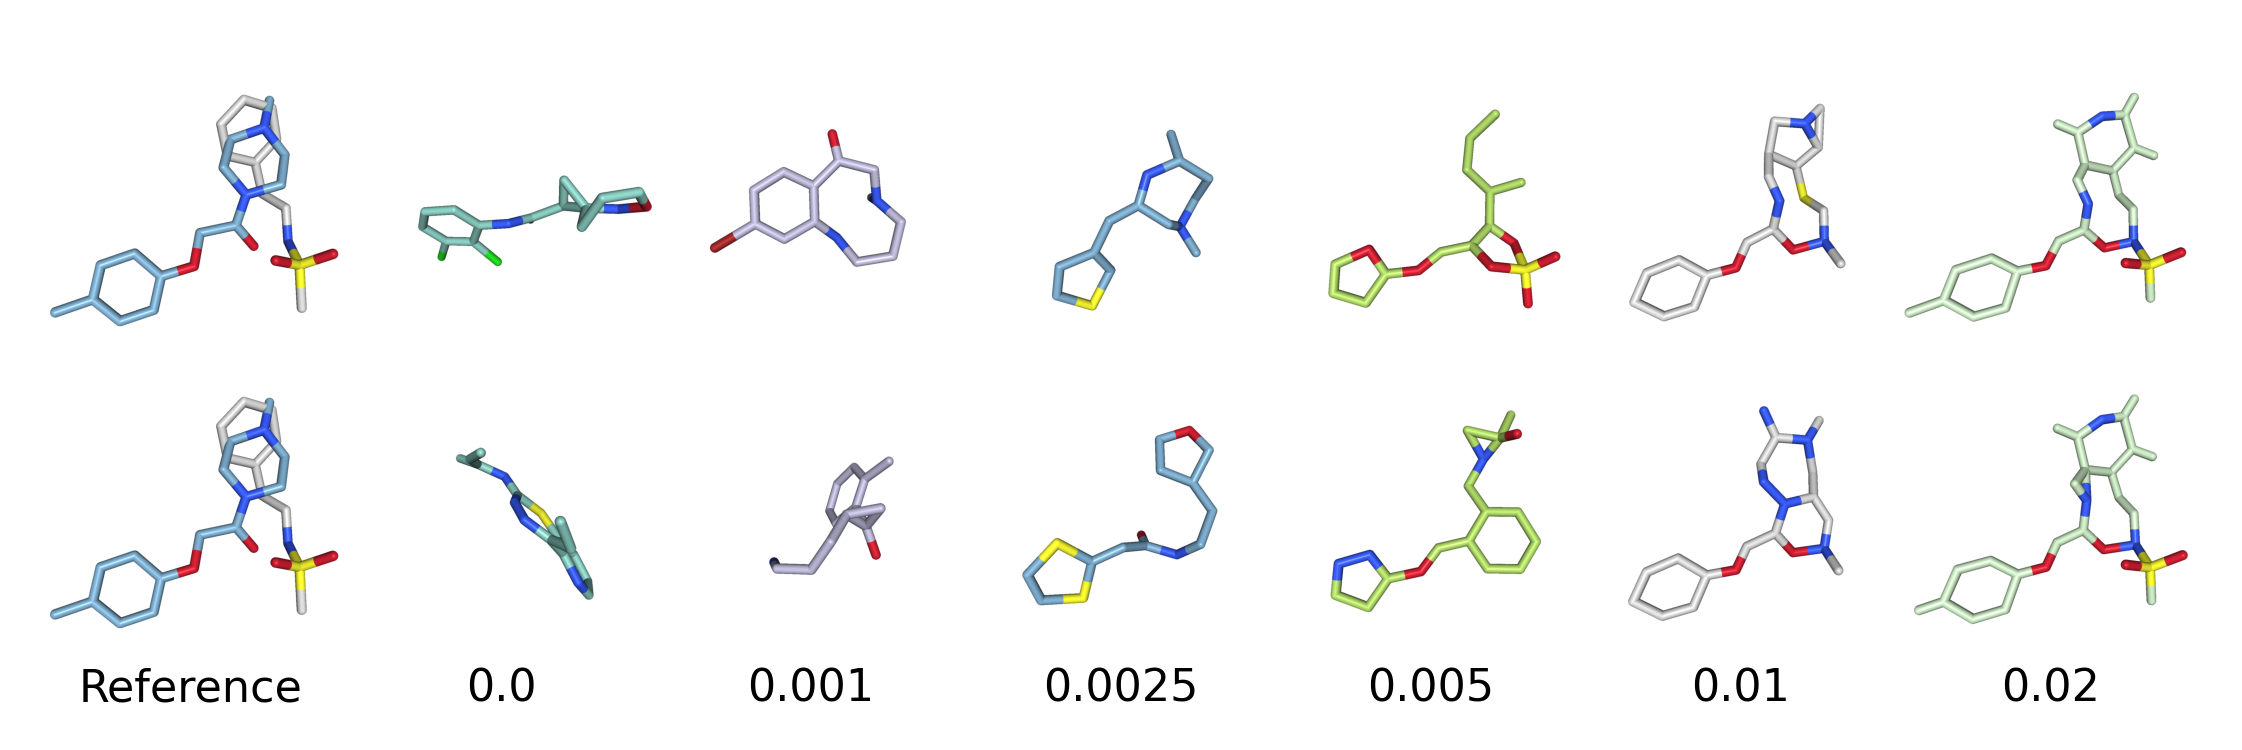
\includegraphics[width=\textwidth]{Figures/molecules_silvr_rates_horizontal.png}
    \caption{This looks much better than I thought}
    \label{fig:fig_2}
\end{figure}


\end{suppinfo}